\DocumentMetadata{
 lang=en,
 testphase={phase-III,math,table,title,firstaid},
 pdfversion=2.0,
 pdfstandard=ua-2,
 pdfstandard=a-4f,
 uncompress
}
\documentclass{book}

\usepackage{titlesec}

\usepackage[linktocpage=true]{hyperref}

\usepackage{caption}
\usepackage{subcaption}
\usepackage{graphicx}



\RemoveFromHook{begindocument}[latex-lab-testphase-float]
\makeatletter
\ExplSyntaxOn
\socket_new_plug:nnn{tagsupport/parbox/before}{caption}
  {   
   \tagpdfparaOn %restart para tagging
   \tl_if_empty:NTF\@current@float@struct
    {     
     \tag_struct_begin:n{tag=Caption,firstkid}
    }
    {
     %\tag_struct_begin:n{tag=Caption,firstkid}
     \tag_struct_begin:n{tag=Caption,parent=\@current@float@struct,firstkid}
    } 
  }
\socket_new_plug:nnn{tagsupport/parbox/after}{caption}
  {
   \tag_struct_end:   
  }
\l@addto@macro\caption@beginex@hook{%
  \tagpdfparaOff %leavevmode in parbox should not start paragraph structure
  \AssignSocketPlug{tagsupport/parbox/before}{caption}
  \AssignSocketPlug{tagsupport/parbox/after}{caption}}
\ExplSyntaxOff
\AtBeginDocument{
	\renewcommand*\caption@anchor[1]{%
        \ifmeasuring@ \else
           \caption@raisedlink{\MakeLinkTarget*{#1}}%
        \fi}%  
}


\ExplSyntaxOn
\cs_new_eq:NN \origsubfigure \subfigure 
\cs_new_eq:NN \origsubfigureend \endsubfigure
\RenewDocumentCommand{\subfigure}{O{b} O{} O{s} m}{
  \origsubfigure[#1][#2][#3]{#4}
  \tagstructbegin{tag=Part}
  \tl_set:Ne\@current@float@struct{\tag_get:n{struct_num}}
}
\ExplSyntaxOff
\def\endsubfigure{
  \tagstructend
  \origsubfigureend
}
\makeatother




\begin{document}
\begin{figure}[!ht]
  \centering
  \begin{subfigure}[b]{0.4\textwidth}
    % \tagstructbegin{tag=Part}
    % \makeatletter
    % \ExplSyntaxOn
    % \tl_set:Ne\@current@float@struct{\tag_get:n{struct_num}}
    % \ExplSyntaxOff
    % \makeatother
    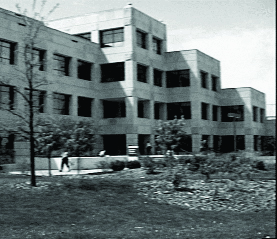
\includegraphics[alt={On top, there is a stacked row of lines.
          From the top, the left and right third of a bar is kept, while the middle third is removed as the lines go down.
          On bottom, the CDF is shown, taking on a rough staircase look with the middle third represented by flat plateaus.
        },width=\textwidth]{Images/dc5.jpg}
    \subcaption{adcd}
    % \tagstructend
  \end{subfigure}
  \hfill
  \begin{subfigure}[b]{0.4\textwidth}
    % \tagstructbegin{tag=Part}
    % \makeatletter
    % \ExplSyntaxOn
    % \tl_set:Ne\@current@float@struct{\tag_get:n{struct_num}}
    % \ExplSyntaxOff
    % \makeatother
    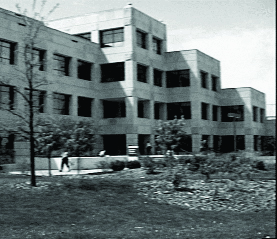
\includegraphics[alt={On top, there is a stacked row of lines.
          From the top, the left and right third of a bar is kept, while the middle third is removed as the lines go down.
          On bottom, the CDF is shown, taking on a rough staircase look with the middle third represented by flat plateaus.
        },width=\textwidth]{Images/dc5.jpg}
    \subcaption{abcd}
    %\tagstructend
  \end{subfigure}
  %\tagmcend

  \caption{abcd}
\end{figure}

\begin{figure}
  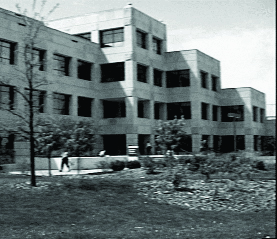
\includegraphics{Images/dc5.jpg}
  \caption{plainAndSimple}
\end{figure}
% \ExplSyntaxOff
% \ResumeTagging
\end{document}